% GNUPLOT: LaTeX picture with Postscript
\begingroup
  \makeatletter
  \providecommand\color[2][]{%
    \GenericError{(gnuplot) \space\space\space\@spaces}{%
      Package color not loaded in conjunction with
      terminal option `colourtext'%
    }{See the gnuplot documentation for explanation.%
    }{Either use 'blacktext' in gnuplot or load the package
      color.sty in LaTeX.}%
    \renewcommand\color[2][]{}%
  }%
  \providecommand\includegraphics[2][]{%
    \GenericError{(gnuplot) \space\space\space\@spaces}{%
      Package graphicx or graphics not loaded%
    }{See the gnuplot documentation for explanation.%
    }{The gnuplot epslatex terminal needs graphicx.sty or graphics.sty.}%
    \renewcommand\includegraphics[2][]{}%
  }%
  \providecommand\rotatebox[2]{#2}%
  \@ifundefined{ifGPcolor}{%
    \newif\ifGPcolor
    \GPcolortrue
  }{}%
  \@ifundefined{ifGPblacktext}{%
    \newif\ifGPblacktext
    \GPblacktexttrue
  }{}%
  % define a \g@addto@macro without @ in the name:
  \let\gplgaddtomacro\g@addto@macro
  % define empty templates for all commands taking text:
  \gdef\gplbacktext{}%
  \gdef\gplfronttext{}%
  \makeatother
  \ifGPblacktext
    % no textcolor at all
    \def\colorrgb#1{}%
    \def\colorgray#1{}%
  \else
    % gray or color?
    \ifGPcolor
      \def\colorrgb#1{\color[rgb]{#1}}%
      \def\colorgray#1{\color[gray]{#1}}%
      \expandafter\def\csname LTw\endcsname{\color{white}}%
      \expandafter\def\csname LTb\endcsname{\color{black}}%
      \expandafter\def\csname LTa\endcsname{\color{black}}%
      \expandafter\def\csname LT0\endcsname{\color[rgb]{1,0,0}}%
      \expandafter\def\csname LT1\endcsname{\color[rgb]{0,1,0}}%
      \expandafter\def\csname LT2\endcsname{\color[rgb]{0,0,1}}%
      \expandafter\def\csname LT3\endcsname{\color[rgb]{1,0,1}}%
      \expandafter\def\csname LT4\endcsname{\color[rgb]{0,1,1}}%
      \expandafter\def\csname LT5\endcsname{\color[rgb]{1,1,0}}%
      \expandafter\def\csname LT6\endcsname{\color[rgb]{0,0,0}}%
      \expandafter\def\csname LT7\endcsname{\color[rgb]{1,0.3,0}}%
      \expandafter\def\csname LT8\endcsname{\color[rgb]{0.5,0.5,0.5}}%
    \else
      % gray
      \def\colorrgb#1{\color{black}}%
      \def\colorgray#1{\color[gray]{#1}}%
      \expandafter\def\csname LTw\endcsname{\color{white}}%
      \expandafter\def\csname LTb\endcsname{\color{black}}%
      \expandafter\def\csname LTa\endcsname{\color{black}}%
      \expandafter\def\csname LT0\endcsname{\color{black}}%
      \expandafter\def\csname LT1\endcsname{\color{black}}%
      \expandafter\def\csname LT2\endcsname{\color{black}}%
      \expandafter\def\csname LT3\endcsname{\color{black}}%
      \expandafter\def\csname LT4\endcsname{\color{black}}%
      \expandafter\def\csname LT5\endcsname{\color{black}}%
      \expandafter\def\csname LT6\endcsname{\color{black}}%
      \expandafter\def\csname LT7\endcsname{\color{black}}%
      \expandafter\def\csname LT8\endcsname{\color{black}}%
    \fi
  \fi
    \setlength{\unitlength}{0.0500bp}%
    \ifx\gptboxheight\undefined%
      \newlength{\gptboxheight}%
      \newlength{\gptboxwidth}%
      \newsavebox{\gptboxtext}%
    \fi%
    \setlength{\fboxrule}{0.5pt}%
    \setlength{\fboxsep}{1pt}%
    \definecolor{tbcol}{rgb}{1,1,1}%
\begin{picture}(7200.00,4320.00)%
    \gplgaddtomacro\gplbacktext{%
      \csname LTb\endcsname%%
      \put(634,619){\makebox(0,0)[r]{\strut{}$0.2$}}%
      \csname LTb\endcsname%%
      \put(634,1062){\makebox(0,0)[r]{\strut{}$0.4$}}%
      \csname LTb\endcsname%%
      \put(634,1505){\makebox(0,0)[r]{\strut{}$0.6$}}%
      \csname LTb\endcsname%%
      \put(634,1947){\makebox(0,0)[r]{\strut{}$0.8$}}%
      \csname LTb\endcsname%%
      \put(634,2390){\makebox(0,0)[r]{\strut{}$1$}}%
      \csname LTb\endcsname%%
      \put(634,2833){\makebox(0,0)[r]{\strut{}$1.2$}}%
      \csname LTb\endcsname%%
      \put(634,3276){\makebox(0,0)[r]{\strut{}$1.4$}}%
      \csname LTb\endcsname%%
      \put(634,3719){\makebox(0,0)[r]{\strut{}$1.6$}}%
      \csname LTb\endcsname%%
      \put(731,425){\makebox(0,0){\strut{}$5$}}%
      \csname LTb\endcsname%%
      \put(1347,425){\makebox(0,0){\strut{}$5.5$}}%
      \csname LTb\endcsname%%
      \put(1962,425){\makebox(0,0){\strut{}$6$}}%
      \csname LTb\endcsname%%
      \put(2578,425){\makebox(0,0){\strut{}$6.5$}}%
      \csname LTb\endcsname%%
      \put(3193,425){\makebox(0,0){\strut{}$7$}}%
      \csname LTb\endcsname%%
      \put(3809,425){\makebox(0,0){\strut{}$7.5$}}%
      \csname LTb\endcsname%%
      \put(4424,425){\makebox(0,0){\strut{}$8$}}%
      \csname LTb\endcsname%%
      \put(5039,425){\makebox(0,0){\strut{}$8.5$}}%
      \csname LTb\endcsname%%
      \put(5655,425){\makebox(0,0){\strut{}$9$}}%
      \csname LTb\endcsname%%
      \put(6270,425){\makebox(0,0){\strut{}$9.5$}}%
      \csname LTb\endcsname%%
      \put(6886,425){\makebox(0,0){\strut{}$10$}}%
    }%
    \gplgaddtomacro\gplfronttext{%
      \csname LTb\endcsname%%
      \put(170,2169){\rotatebox{-270}{\makebox(0,0){\strut{}$U_0/\SI{}{V}$}}}%
      \csname LTb\endcsname%%
      \put(3809,135){\makebox(0,0){\strut{}$\nu / \SI{}{10^{14} Hz}$}}%
      \csname LTb\endcsname%%
      \put(6123,1083){\makebox(0,0)[r]{\strut{}$U_0$ Datenpunkte}}%
      \csname LTb\endcsname%%
      \put(6123,890){\makebox(0,0)[r]{\strut{}$f(\nu)=\SI{0.228 +- 0.065}{V/\ 10^{14} Hz}\cdot \nu \SI{-0.90 +- 0.45}{V}$}}%
      \csname LTb\endcsname%%
      \put(3809,4009){\makebox(0,0){\strut{}$W_A=\SI{-0.90 +- 0.45}{eV}$, $\text{h}=\SI{0.0228 +- 0.0065 }{eVs} \cdot 10^{-15} $ und $\chi^2/\text{ddof}=752.338$}}%
    }%
    \gplbacktext
    \put(0,0){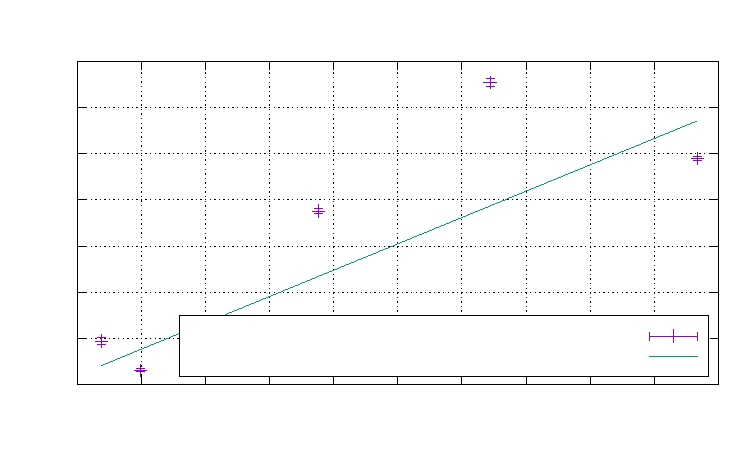
\includegraphics[width={360.00bp},height={216.00bp}]{Austritsarbeit}}%
    \gplfronttext
  \end{picture}%
\endgroup
